\documentclass[parskip=full]{scrartcl}

\pdfoutput=1

\usepackage{breakcites}
\usepackage[square,numbers]{natbib}
\usepackage{float}
\usepackage{graphicx}
\usepackage{geometry}
\geometry{%
	a4paper,
	left=18mm,
	right=18mm,
	top=18mm,
}
\usepackage{amsmath}
\usepackage{enumitem}
\usepackage[ruled,vlined]{algorithm2e}
\usepackage{booktabs}
\usepackage{pgfplotstable}
\pgfplotsset{compat=1.14}
\usepackage{longtable}
\usepackage{tabu}
\usepackage{hyperref}
\date{}

\definecolor{hypecol}{HTML}{0875b7}
\hypersetup{%
    colorlinks,
    linkcolor={hypecol},
    citecolor={hypecol},
    urlcolor={hypecol}
}

\title{%
    Research Trends and Applications of Data Augmentation Algorithms
}

\author{%
	Joao Fonseca\(^{1*}\), Fernando Bacao\(^{1}\)
	\\
	\small{\(^{1}\)NOVA Information Management School, Universidade Nova de Lisboa}
	\\
	\small{*Corresponding Author}
	\\
	\\
	\small{Postal Address: NOVA Information Management School, Campus de
    Campolide, 1070--312 Lisboa, Portugal}
	\\
	\small{Telephone: +351 21 382 8610}
}

\begin{document}

\maketitle

\section{Introduction}

Introduction goes here.

\section{Theory}

This part is going to be the very last thing to be done, since it doesn't seem
absolutely necessary.

\section{Methodology}

In this section we describe the procedures defined for the literature
collection, data preprocessing and literature analysis. The analysis of the
literature was developed with 3 different approaches. Throughout the
analyses, data preprocessing and hyperparameter tuning was developed
iteratively. The procedure adopted in this manuscript is shown in
Figure~\ref{fig:slr_diagram}.

The analysis and modelling was developed using the Python programming
language, along with the
\href{https://scikit-learn.org/stable/}{Scikit-Learn}~\cite{Pedregosa2011},
\href{https://radimrehurek.com/gensim/}{Gensim}~\cite{Rehurek2010},
\href{https://github.com/lmcinnes/umap}{Umap-Learn}~\cite{Mcinnes2018} and
\href{https://networkx.org/}{Networkx}~\cite{Hagberg2008} libraries. The final
network analysis and visualization was done with
\href{https://gephi.org/}{Gephi}~\cite{Bastian2009}. 

An exploratory data analysis was done to understand which manuscripts, journals
and conferences are most significant within the field of Data Augmentation. 

Text Mining perspective

\begin{itemize}
    \item General overview of the steps taken to produce the visualizations
        and analyses.
    \item Use diagrams and visualizations.
    \item Discuss embedding techniques used.
\end{itemize}

\begin{figure}[H]
	\centering
	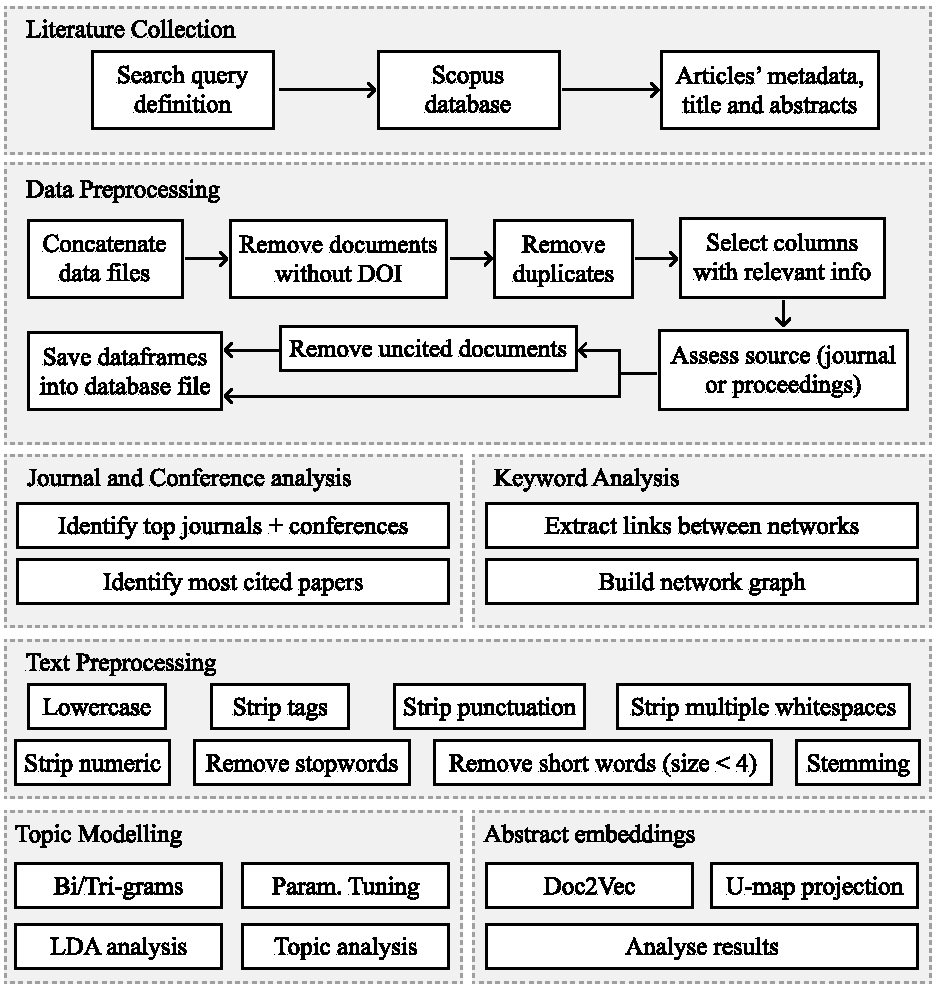
\includegraphics[width=.75\linewidth]{../analysis/slr_diagram}
    \caption{Diagram of the proposed literature analysis approach.
    }~\label{fig:slr_diagram}
\end{figure}

\subsection{Keyword Identification and Search}

The focus of this literature analysis is to understand the different
algorithms, domains and/or tasks that employ data augmentation techniques.
Therefore, we use the keyword ``data augmentation'' in order to ensure an
unbiased analysis. The results were then limited to conference papers and
journal articles written in English that were published in the past 15 years.
Due to the already large amount of results found, the document retrieval was
done using solely the \href{https://www.scopus.com/}{Scopus} database. The
resulting query is shown below:

\begin{verbatim}
    KEY ( "data augmentation" )  AND  ( LIMIT-TO ( LANGUAGE ,  "English" ) )  
    AND ( LIMIT-TO ( DOCTYPE ,  "cp" )  OR  LIMIT-TO ( DOCTYPE ,  "ar" ) )  
    AND  (
            LIMIT-TO ( PUBYEAR ,  2021 )  OR  LIMIT-TO ( PUBYEAR ,  2020 )  
        OR  LIMIT-TO ( PUBYEAR ,  2019 )  OR  LIMIT-TO ( PUBYEAR ,  2018 )  
        OR  LIMIT-TO ( PUBYEAR ,  2017 )  OR  LIMIT-TO ( PUBYEAR ,  2016 )  
        OR  LIMIT-TO ( PUBYEAR ,  2015 )  OR  LIMIT-TO ( PUBYEAR ,  2014 )  
        OR  LIMIT-TO ( PUBYEAR ,  2013 )  OR  LIMIT-TO ( PUBYEAR ,  2012 )  
        OR  LIMIT-TO ( PUBYEAR ,  2011 )  OR  LIMIT-TO ( PUBYEAR ,  2010 )  
        OR  LIMIT-TO ( PUBYEAR ,  2009 )  OR  LIMIT-TO ( PUBYEAR ,  2008 )  
        OR  LIMIT-TO ( PUBYEAR ,  2007 )  OR  LIMIT-TO ( PUBYEAR ,  2006 ) 
    )  
\end{verbatim}



Started with a single keyword: ``Data Augmentation'', 4618 results.

Limited results to documents written in English, 4517 results.

Only include articles and conference papers, 4443 results.

Consider papers published in the past 15 years, 4281 results.

Final query:

Due to the limitations in the Scopus data export (maximum 2000 documents per
export), the data was extracted in four parts: 2021, 2020, 2019 and 2018 --- 2006.

One of the exported references had a corrupted line, which caused the loss of one
additional document.

Removed references without a DOI, 3948 results.

Removed references without a single citation, 2259 results. Exception made for
journals and conference analysis.  



For the network analysis:

Out of the 2259 results, 1923 contained keywords in Scopus' database.

Keyword combinations showing up in only one document are removed from further
analysis.

The network consists of an undirected graph whose weights consist of the
following formula: $Keyword--pair weight = \log(Avg cites * Nbr of documents)$
to avoid a disproportional bias of highly cited research articles.


\subsection{Repositories}

\begin{itemize}
    \item Repositories: Scopus
\end{itemize}

\subsection{Bibliometric Analysis}

\begin{itemize}
    \item Discuss data preprocessing done.
    \item Concatenate data, extract features (if possible), data cleaning etc
\end{itemize}

\subsection{Data Analysis Software for Bibliometric Research}

\begin{itemize}
    \item Python
    \item Streamlit
    \item Text Mining and Embedding libraries
    \item Data Visualization libraries
    \item VOSviewer?
\end{itemize}

\section{Results}

Results go here.

\subsection{PRISMA Flow Diagram}

\begin{itemize}
    \item Create a flowchart with the data cleaning process and describe it.
\end{itemize}

\subsection{Terms Frequency}

\subsection{Topics Discovered}

LDA analysis goes here

\subsubsection{Main Journals}

\subsubsection{Main Conference Proceedings}

\subsection{Author Co-occurrence Analysis}

Not sure whether to keep this one.

\subsection{Title and Abstract Text Occurrence Analysis}

This can be done by text occurrence network visualization or embedings

\subsection{Most Cited Publications}

\subsection{Application and Method Analysis}

\section{Discussion}

Discussion goes here.

\subsection{Research Question Discussion}

\subsection{Research Gap Discussion}

\subsection{Study Limitation Discussion}

\section{Conclusions}

\bibliography{references}
% \bibliographystyle{apalike}
\bibliographystyle{ieeetr}

\end{document}
